\chapter{Introduction}

\section{Motivation}
Project driven organizations face the problem of constantly needing to put teams together based on the members’ skills, experience and preferences.
In many businesses, there is no adequate source of information about those data which makes finding the right person with a specific ability even more complicated. A popular approach to this problem is using computer programs to find an employee skilled in a given set of tasks in all available employees.

SinnerSchrader, a Hamburg based web agency that will serve as the practical context for this thesis, decided to launch an internal application for skills management that is meant to solve the aforesaid problems. This thesis will deal with the design, concept, partial implementation and evaluation of said application.



\subsection{SinnerSchrader}

The SinnerSchrader Group is a full-service web agency based in Hamburg aggregating the subcompanies SinnerSchrader Deutschland, SinnerSchrader Content, SinnerSchrader Commerce and SinnerSchrader Swipe. The broad spectrum of expertise, including, but not limited to, digital communication strategies, visual and interaction design,  technical architecture, full stack development, editorial services, content production, e-commerce, mobile app development, hosting, and maintenance, allows SinnerSchrader to serve all needs regarding their customers' digital transformation. The combination of all said competencies under one single roof reduces organizational friction between the discipline-specific teams because they all share the same vision of the big picture they are creating. This does not only lead to faster development cycles but also to a more coherent and unified product.
If not stated otherwise, the name \textit{SinnerSchrader} will further refer to SinnerSchrader Deutschland.

\newpage

\subsubsection{Project-Driven Business}
Being a web agency, SinnerSchrader operates in a project-driven way. This means there is no continuous stream of recurring work repeating constantly, but many different projects for different clients, each one dealing with varying challenges and questions. From a technical point of view, the diversity of know-how needed for each project is extremely huge since every application uses its own dedicated stack of technologies. As a consequence, the developers’ skill sets are based on the combination of projects they have worked on and their general field of interest. This results managers frequently having to put teams together based on the members’ skills with respect to the individual requirements of the project.

\subsubsection{Matrix organization}
The personnel of SinnerSchrader is divided into two different types of teams: functional teams of
employees sharing the same specialization, e.g. backend development, frontend development, design, business strategy, or concept, and project teams of people from different functional teams working collaboratively on the same project. This structural model is called a matrix organization \cite[P. 75]{BWL}.
The organizational head of functional teams will further be called the \textit{supervisor} the pendant for project team will be mentioned as \textit{team manager}.

\begin{figure}[!htp]
    \centering
    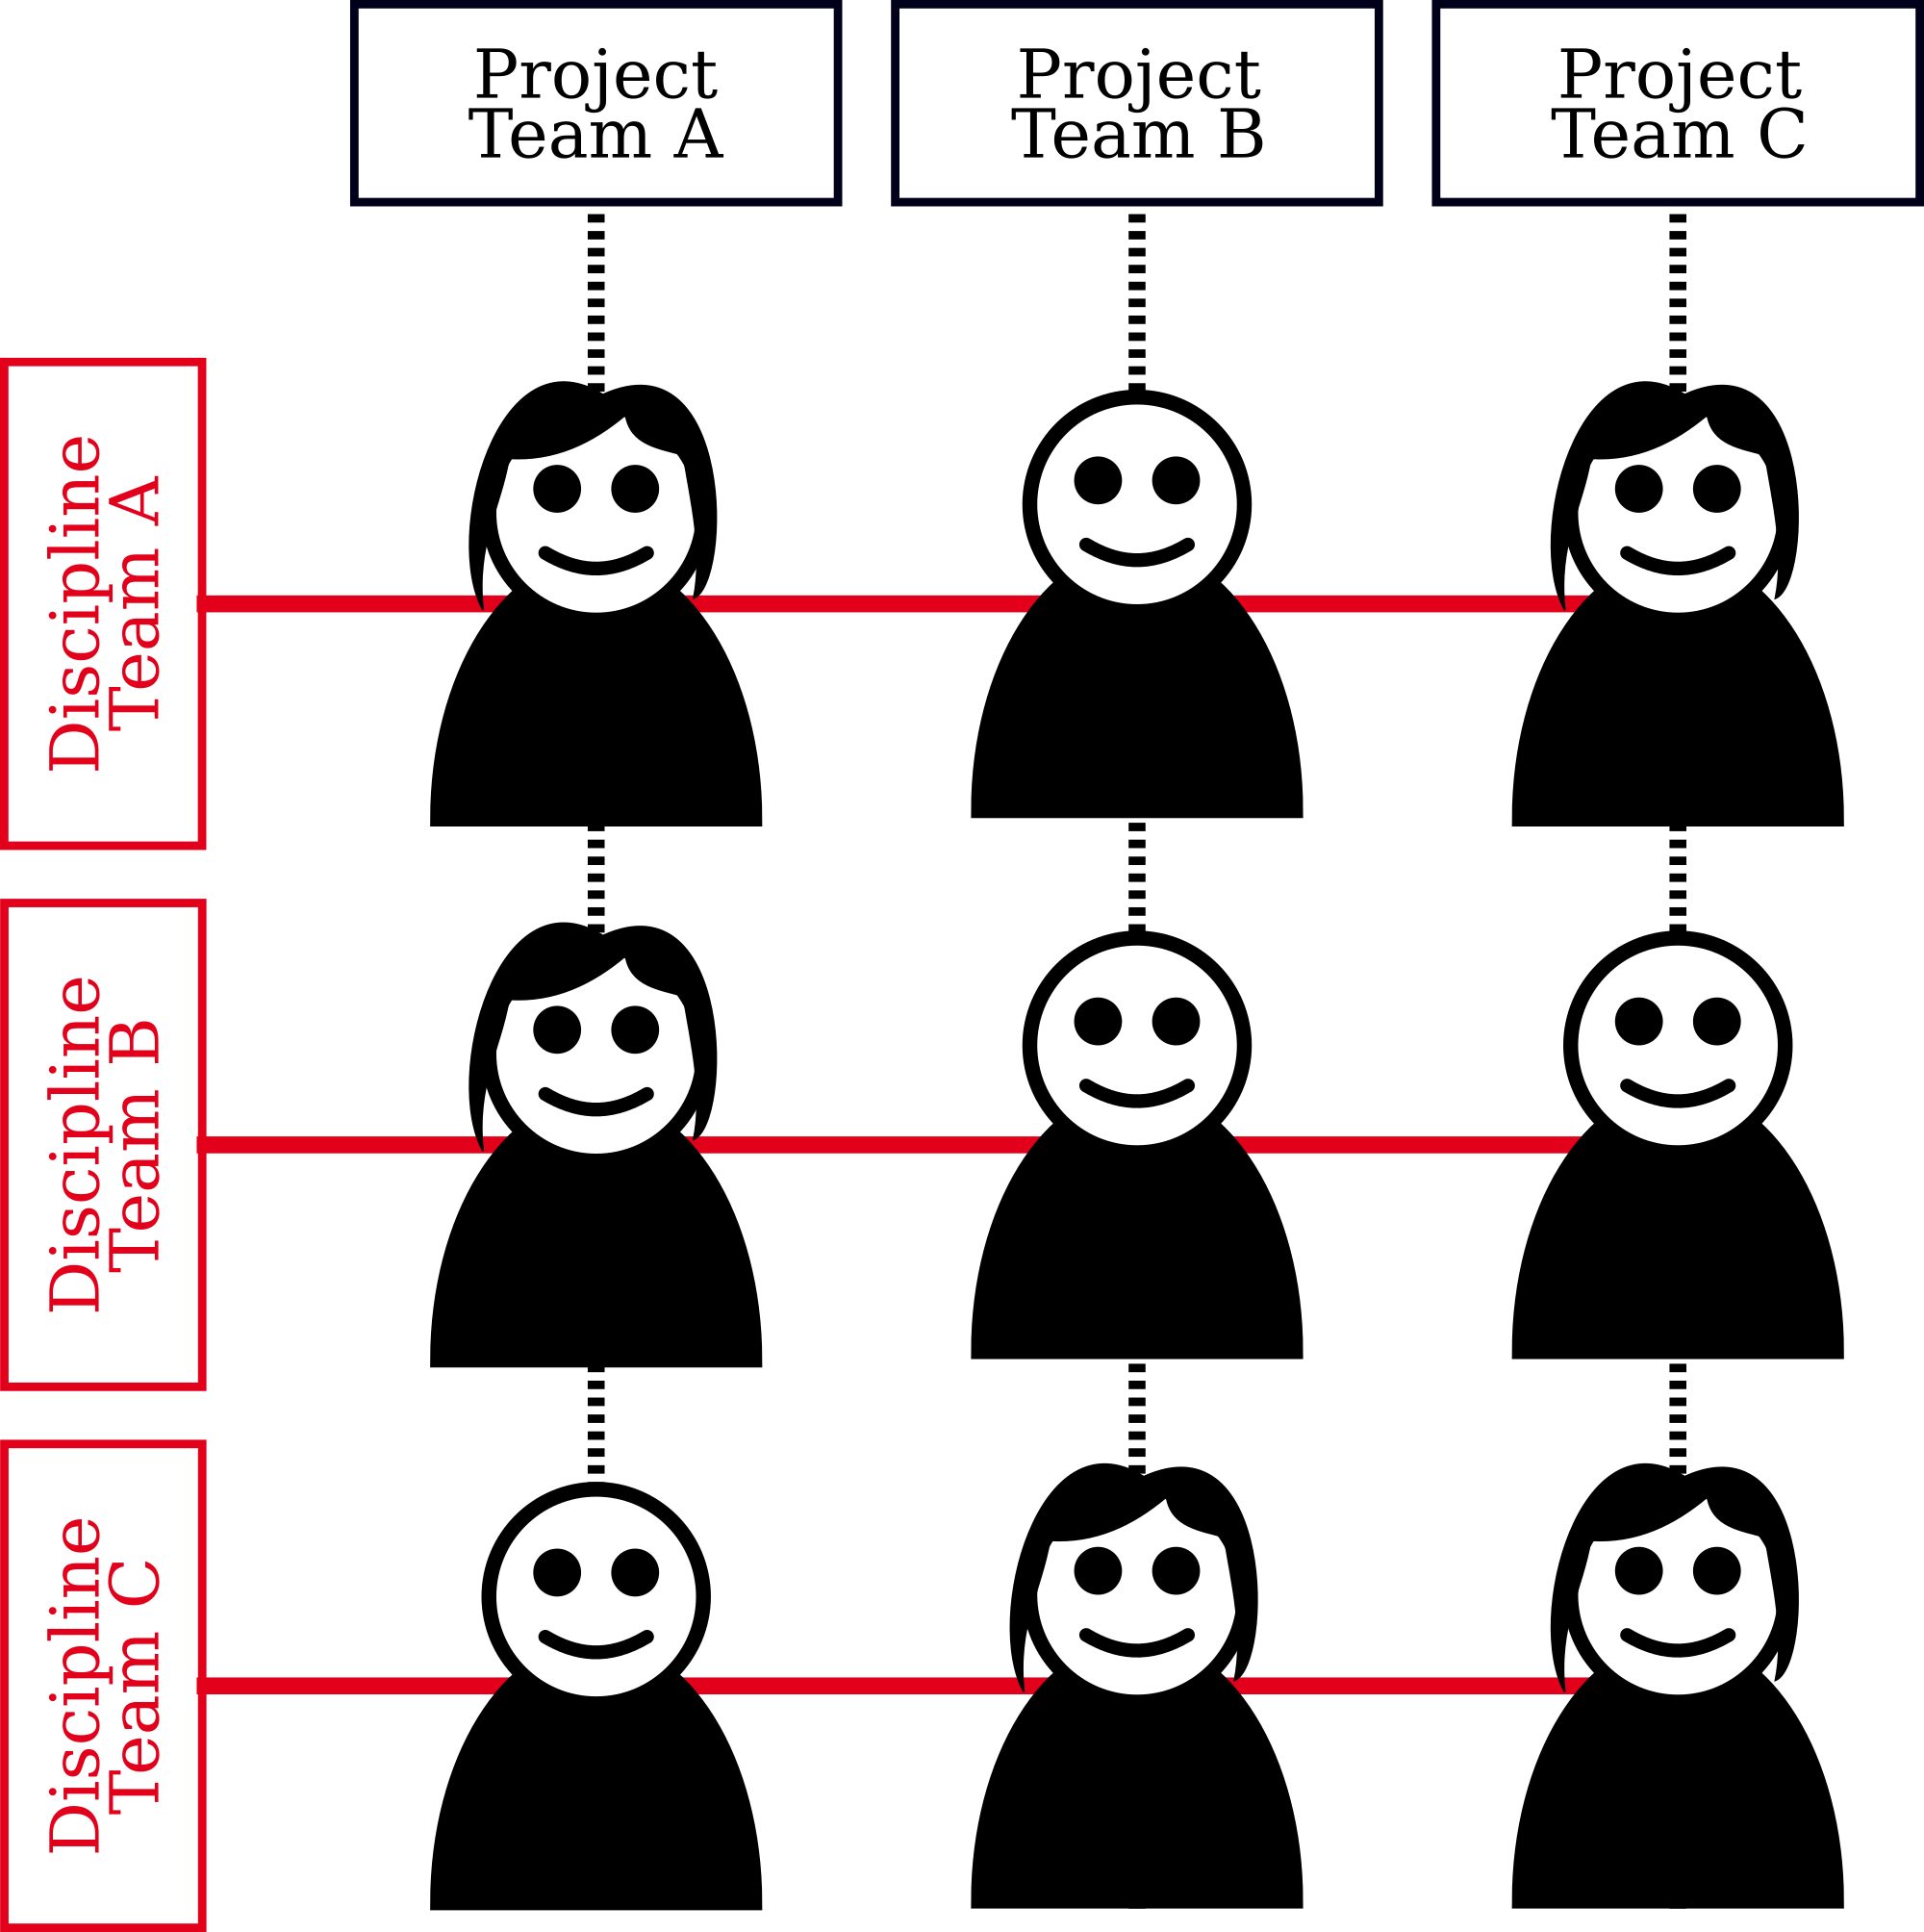
\includegraphics[width=0.5\textwidth]{images/matrixorga.png}
    \caption[Diagram: Matrix organization]{Illustration of a matrix organization}
    \label{fig:matrixorga}
\end{figure}

\newpage

\section{Leading Goals}
The main goal of this thesis is to design, partially implement, and evaluate a skills management application custom-tailored to SinnerSchrader using a novel approach to search for employees. Instead of returning the most skilled persons, the tool will list the most suitable ones employing a ranking mechanism that measures how well someone fits into the searched skill set. An analysis of the user's expectations will be used to define \textit{suitability} in this context.
Furthermore, recommender systems that enrich the user experience will be evaluated, designed, and implemented.
The created methods and implementations will be evaluated both technically and conceptually.
